In questa capitolo si descriverà il problema affrontato per poi passare alle versioni sequenziale e distribuita della soluzione, e infine si discuterà delle prestazioni delle due versioni.
\newline
\section{Descrizione del problema}

Il problema affrontato in questo studio riguarda l' applicazione dell'algoritmo \textbf{SIFT}(Scale-Invariant Feature Transform) per effettuare object detection. L' object detection è una tecnologia informatica correlata alla visione artificiale e all'elaborazione di immagini che si occupa di rilevare istanze di oggetti semantici di una determinata classe in immagini e video digitali. Il rilevamento di oggetti ha applicazioni in molte aree della visione artificiale, tra cui il recupero di immagini e la videosorveglianza. 
Per ogni oggetto in un'immagine, ci sono molte features, che sono caratteristiche interessanti dell'oggetto, le quali possono essere estratte in modo da fornire una descrizione "caratteristica" dell'oggetto. Questa descrizione estratta da una immagine campione può poi essere utilizzata per identificare l'oggetto durante il tentativo di individuare l'oggetto in una immagine contenente più oggetti. Per poter recuperare queste features esistono diversi algoritmi quali per esempio SURF(Speeded Up Robust Features), ORB (Oriented FAST and Rotated BRIEF) e SIFT in questo studio ci siamo concentrati su quest'ultimo il quale è un algoritmo cpu-intensive e quindi ci interessava analizzare il suo comportamento in un ambiente distribuito.

\subsection{SIFT}
Scale-invariant feature transform (SIFT) è un algoritmo utilizzato in computer vision che permette di rilevare e descrivere caratteristiche pubblicato da David G. Lowe\site{lowe04} nel 2004.
L'algoritmo consiste in un metodo in grado di estrarre delle caratteristiche distintive invarianti da un immagine che possono essere utilizzate per effettuare un matching tra diversi oggetti. Le caratteristiche sono invarianti rispetto alla scala e alla rotazione dell'immagine e sono mostrate per fornire una robusta corrispondenza su una vasta gamma di distorsioni affini, cambiamenti nel punto di vista 3D, aggiunta di rumore e cambiamento nell'illuminazione. L'algoritmo esegue cinque step:
\begin{itemize}
\item \textbf{Scale-space Extrema Detection}
Per poter individuare dei keypoints abbiamo bisogno di diverse scale di un immagine quindi viene applicato un filtro per la scala. Questo filtro utilizza Laplaciana di una Gaussiana(LoG) che permette di rilevare blob di varie dimensioni grazie all'utilizzo $\sigma$ che funge come parametro di scala. Poichè LoG è costoso SIFT usa la differenza gaussiana(DoG) come alternativa che è una approssimazione del primo. La DoG è ottenuta come differenza di sfocatura gaussiana di un immagine con diversi $\sigma$ (si parte da un valore iniziale di $\sigma$ fino ad arrivare $k\sigma$) . Questo processo viene eseguito per diverse ottave dell'immagine.

\begin{figure}[!h]
	\begin{center}
    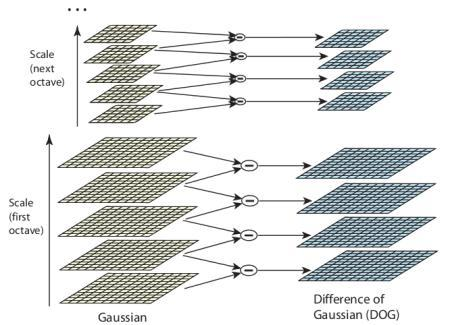
\includegraphics[scale=0.4]{DoG.jpg}
    \caption{Ottave di un immagine}
    \label{fig:DoG}
    	\end{center}
\end{figure}

Una volta trovato DoG vengono cercati i keypoints che rappresentano meglio l'immagine confrontando i pixel su diverse scale, per esempio un pixel in una immagine viene confrontato con i suoi 8 vicini e e con i 9 pixel della scala precedente e successiva.

\begin{figure}[!h]
  \begin{center}
    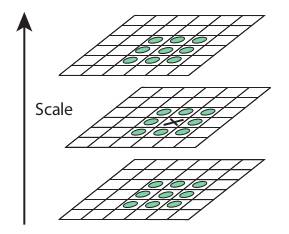
\includegraphics[scale=0.5]{kp.jpg}
    \caption{Ricerca di un keypoints}
    \label{fig:kp}
    	\end{center}
\end{figure}

%Il paper fornisce alcuni dati ottimali e sono: numero di ottave = 4, livelli di scala = 5 valore iniziale $\sigma$ = 1.6 e k = 2-$\sqrt$.

\item \textbf{Keypoint Localization}

Una volta individuati potenziali keypoints, devono essere affinati per ottenere risultati più accurati. Viene usata l'espansione della serie di Taylor dello spazio di scala per ottenere una posizione più accurata dei punti e, se l'intensità di un punto è inferiore a un valore di threshold (0,03 valore di soglia del paper), viene rifiutata.

La DoG(Difference of Gaussian) ha una risposta più alta per gli edge e che quindi vanno rimossi, per fare questo SIFT usa una matrice Hessiana 2x2 per computare la curvatura per poi confrontarla con la threshold degli edge se viene superata allora gli edge vengono rimossi
\item \textbf{Orientation Assignment}

Successivamente viene assegnato un orientamento a ciascun keypoint per ottenere l'invarianza alla rotazione dell'immagine. Dei vicini vengono presi attorno alla posizione del punto in base alla scala, e al modulo del gradiente e la direzione vengono calcolate in quella regione. Viene creato un istogramma di orientamento con 36 contenitori a 360 gradi. Viene pesato per il modulo del gradiente e la gaussian-weighted circular window con $\sigma$ uguale a 1,5 volte la scala del punto chiave, viene preso il picco più alto nell'istogramma e anche qualsiasi picco superiore a 80 vengono considerati per calcolare l'orientamento.
\item \textbf{Keypoint Descriptor}

In questa fase viene creato un descrittore di keypoint. Viene preso un intorno 16x16 attorno al keypoint. Viene  diviso in 16 sotto blocchi di dimensione 4x4. Per ciascun sottoblocco viene creato un istogramma di orientamento a 8 bin. Quindi sono disponibili in totale 128 valori bin. Questo rappresentato come un vettore per formare un descrittore di keypoints. Oltre a questo, vengono prese diverse misure per ottenere robustezza contro i cambiamenti di illuminazione, la rotazione ecc.


\item \textbf{Keypoint Matching}

I keypoints tra due immagini sono abbinati identificando i loro vicini più vicini. Ma in alcuni casi, la seconda corrispondenza più vicina potrebbe essere molto vicina alla prima. Questo può accadere a causa di rumore o per altri motivi. In questi casi, viene preso il rapporto tra distanza più vicina e distanza più vicina al secondo. Se è maggiore di 0.8, vengono rifiutati. In questo modo si riesco a elimianre circa il 90\% di false corrispondenze mentre scarta solo il 5\% corrispondenze corrette.
	


\end{itemize}

\subsection{OpenCV}

Per l'implementazione dell' object detection è stato utilizzato OpenCV. OpenCV (Open Source Computer Vision Library) è una libreria open source di computer vision e di apprendimento automatico, realizzato per fornire un'infrastruttura comune per le applicazioni di visione artificiale e per accelerare l'uso della percezione della macchina nei prodotti commerciali. OpencCV è rilasciato con licenza BSD

\noindent La libreria ha più di 2500 algoritmi ottimizzati, che comprendono un set completo di algoritmi di visione artificiale e di apprendimento automatico sia classici che all'avanguardia. questi algoritmi possono essere utilizzati per rilevare e riconoscere i volti, identificare gli oggetti, classificare azioni umane nei video, tracciare i movimenti della telecamera, tracciare oggetti in movimento, estrarre modelli 3D di oggetti, trova immagini simili da un database di immagini, rimuovi gli occhi rossi dalle immagini scattate con il flash, segui i movimenti degli occhi, riconosci i paesaggi e stabilisci i marcatori per sovrapporli alla realtà aumentata, ecc.

\noindent OpenCV supporta diversi linguaggi C++, Python, Java e MATLAB e i pricipali sistemi operativi Linux, Windows Mac os, e Android.

\section{Versione Sequenziale}
La versione sequenziale prevede l'individuazione di un unico oggetto(query) all'interno di una o più scene(train). Prima estrae le caratteristiche grazie all'algoritmo SIFT dall'immagine query e dall'immagine di train, successivamente viene effettuato il match tra le due immagini utilizzando l'algoritmo di Brute Force fornito da OpenCV, e infine viene disegnata l'omografia in caso di match positivo.



\begin{lstlisting}

\end{lstlisting}

Descrizione della risoluzione del problema in ambiente shared memory.
\section{Versione Distibuita con Hadoop}
Descrizione della versione distribuita con Hadoop
\section{Analisi delle prestazioni}
%TODO fare weak scaling e strong scaling
Vengono forniti i benchmark con rispettive spiegazioni
